%==============================================================================
% Poster bachelorproef - De effectiviteit van gamification bij het aanleren
% van COBOL aan junior developers (Learn COBOL)
%==============================================================================
% Gebaseerd op document class `a0poster' door Gerlinde Kettl en Matthias Weiser
% Aangepast voor gebruik aan HOGENT door Jens Buysse en Bert Van Vreckem
% Compileer met XeLaTeX (-shell-escape), zie make_poster.bat/.sh

\documentclass[a0,portrait]{hogent-poster}

% Zoek afbeeldingen zowel in de lokale poster/graphics als in de centrale map
\graphicspath{{graphics/}{../graphics/}}

% Extra pakketten voor opmaak en visualisaties
\usepackage{tikz}
\usetikzlibrary{arrows.meta,positioning,calc}
\usepackage{tabularx}
\usepackage{array}
\usepackage{enumitem}
\usepackage{csquotes}

% Bronverwijzingen: hergebruik de bibliografie van de bachelorproef.
% URL's, DOI's en ISBN's worden weggelaten zodat de referentielijst compact blijft.
\usepackage[backend=biber,style=numeric,sorting=none,maxbibnames=2,giveninits=true,
            url=false,doi=false,isbn=false,eprint=false]{biblatex}
\addbibresource{../bachproef/bachproef.bib}
\renewcommand*{\bibfont}{\scriptsize}
\setlength{\bibitemsep}{2pt}
\setlength{\bibparsep}{0pt}

% Compactere verticale ruimte rond koppen zodat alles op een pagina past
\titlespacing{\section}{0pt}{0.45\baselineskip}{2pt}
\titlespacing{\subsection}{0pt}{0.3\baselineskip}{2pt}
\setlength{\abovecaptionskip}{10pt}

% HoGent-logo dichter bij de rechterrand
\fancypagestyle{plain}{%
  \fancyhf{}%
  \renewcommand{\headrulewidth}{0pt}%
  \fancyfoot[R]{%
    \begin{tikzpicture}[remember picture, overlay]
      \node [anchor=south east, shift={(-1cm, \the\wd\logopart)},
             inner sep=0, outer sep=0] at (current page.south east) {%
        
\includegraphics[height=\the\ht\logopart]{hogent_logo}%
      };%
    \end{tikzpicture}%
  }%
}

% Titel full width; promotor en co-promotor naast elkaar
\makeatletter
\renewcommand{\@maketitle}{%
  \begingroup
  \raggedright\titlefont\color{title}\Large
  \textsc{\@course\ \@studyprogramme\ (\@academicyear)}
  \endgroup

  \begingroup
  \medskip
  \raggedright\titlefont\color{title}\VeryHuge\@title

  \if\@subtitle\@empty\else
    \medskip
    \raggedright\titlefont\Huge\textit{\@subtitle}
  \fi
  \endgroup

  \begingroup
  \bigskip
  \raggedright\huge\textbf{\@author}

  \if\@email\@empty\else
    \medskip
    \raggedright\@email
  \fi
  \endgroup

  \begingroup
  \if\@supervisor\@empty
    \if\@cosupervisor\@empty\else
      \medskip
      \raggedright\Large Co-promotor: \@cosupervisor
    \fi
  \else
    \if\@cosupervisor\@empty
      \medskip
      \raggedright\Large Promotor: \@supervisor
    \else
      \medskip
      \noindent
      \begin{minipage}[t]{0.5\textwidth}
        \raggedright\Large Promotor: \@supervisor
      \end{minipage}%
      \begin{minipage}[t]{0.5\textwidth}
        \raggedright\Large Co-promotor: \@cosupervisor
      \end{minipage}
    \fi
  \fi
  \endgroup

  \begingroup
  \bigskip
  \raggedright\Large\@institution
  \endgroup

  \bigskip
}
\makeatother

% Keuzerichting, sleutelwoorden en broncode in drie kolommen
\makeatletter
\renewenvironment{abstract}
{%
  \bigskip\bigskip
  \addtolength{\leftmargin}{1em}
  \begin{center}
    {\Large\titlefont\abstractname}
  \end{center}
  \list{}{%
    \setlength{\leftmargin}{2cm}
    \setlength{\rightmargin}{\leftmargin}}%
  \item\relax\normalfont\itshape
}{%
  \endlist
  \bigskip
  \noindent\makebox[\textwidth]{%
    \begin{minipage}[t]{0.31\textwidth}
      \centering
      \if\@specialisation\@empty\else
        \if@english Specialisation: \else Keuzerichting: \fi
        \@specialisation
      \fi
    \end{minipage}%
    \hfill
    \begin{minipage}[t]{0.31\textwidth}
      \centering
      \if\@keywords\@empty\else
        \if@english Keywords: \else Sleutelwoorden: \fi
        \@keywords
      \fi
    \end{minipage}%
    \hfill
    \begin{minipage}[t]{0.31\textwidth}
      \centering
      \if\@projectrepo\@empty\else
        \if@english Source code: \else Broncode: \fi
        \url{\@projectrepo}
      \fi
    \end{minipage}%
  }
  \bigskip
}
\makeatother

% Hulpkleuren afgeleid van de HOGENT-huisstijl
\colorlet{accent}{hogent-blue}
\colorlet{accentdark}{hogent-darkgreen}

% Compacte ``stat''-box voor de kerncijfers
\newcommand{\statbox}[3]{%
  \begin{tikzpicture}
    \node[rectangle, rounded corners=10pt, fill=#1, text=white,
          text width=0.40\linewidth, minimum height=3.8cm,
          align=center, inner sep=10pt] {%
      {\huge\titlefont #2}\\[4pt]
      {\footnotesize #3}%
    };
  \end{tikzpicture}%
}

% Info over de opleiding
\course{Bachelorproef}
\studyprogramme{toegepaste informatica}
\academicyear{2025-2026}
\institution{Hogeschool Gent, Valentin Vaerwyckweg 1, 9000 Gent}

% Info over de bachelorproef
\title{De effectiviteit van gamification bij het aanleren van COBOL aan junior developers.}
\subtitle{Learn COBOL, een gamified leerpad voor junior developers}
\author{Silas De Vuyst}
\email{silas.devuyst@student.hogent.be}
\supervisor{Dhr. T. Desmedt}
\cosupervisor{Dhr. S. Willems}

\specialisation{Mainframe}
\keywords{COBOL, gamification, Octalysis, mainframe, junior developers}
\projectrepo{https://github.com/SDeVuyst/BAP-Cobol-Gamification}

\begin{document}

\maketitle

\begin{abstract}
Wereldwijd draaien banken, overheden en zorginstellingen op honderden miljarden regels COBOL, terwijl ervaren specialisten met pensioen gaan en weinig nieuw talent bijkomt. Junior developers groeien op met interactieve, gamified leeromgevingen, maar voor COBOL is dat aanbod er nauwelijks. Deze bachelorproef onderzoekt hoe effectief gamification is bij het aanleren van COBOL aan junioren met een Python-achtergrond. Op basis van een literatuurstudie werd de Proof-of-Concept \textit{Learn COBOL} gebouwd, waarna elke ontwerpkeuze via een vergelijkende literatuurevaluatie tegen bestaand empirisch onderzoek werd afgezet.
\end{abstract}

\begin{multicols}{2}
% Iets compactere bodytekst zodat de volledige poster op een pagina past.
% De sectiekoppen behouden hun grote formaat (titlesec gebruikt absolute groottes).
\small

%==============================================================================
\section{Probleemstelling}

De financiele en publieke sector rust op een fundament van decennia-oude COBOL-code. Naar schatting draaien er nog steeds 250 miljard regels in productie \autocite{IBM2025}, terwijl de \enquote{silver tsunami} de sector treft: ervaren ontwikkelaars gaan massaal met pensioen en de instroom van nieuw talent stagneert \autocite{IBM2025}.

Het echte knelpunt ligt niet enkel bij de taal, maar bij de verouderde didactiek. Moderne talen worden aangeleerd via interactieve sandboxes met directe feedback, terwijl COBOL-onderwijs blijft steken bij statische PDF-handleidingen. Voor een junior met een Python-achtergrond botst dat met de leerverwachtingen, waardoor talent afhaakt nog voor het de logica van het mainframe beheerst.

%------------------------------------------------------------------------------
\subsection{Kerncijfers van de mainframe-context}

\noindent
\statbox{accentdark}{250 mld}{regels COBOL in productie \autocite{IBM2025}}\hfill
\statbox{accent}{$\sim$85\%}{wereldwijd betalingsverkeer via mainframes \autocite{IBM2022a}}\par
\medskip
\noindent
\statbox{hogent-orange}{2,9 $\to$ 5,6}{mld \$ mainframemarkt, 2022 naar 2032 \autocite{Allied2022}}\hfill
\statbox{hogent-purple}{66\%}{mainframe-pros zijn Millennial of Gen Z \autocite{BMC2025}}\par
\medskip

%==============================================================================
\section{Onderzoeksvraag}

\begin{tikzpicture}
  \node[rectangle, rounded corners=12pt, draw=accent, line width=3pt,
        fill=accent!8, text width=0.92\linewidth, align=flush left,
        inner sep=22pt] {%
    \large\itshape Hoe effectief is gamification bij het aanleren van COBOL aan
    junior developers die gewend zijn aan moderne talen zoals Python?%
  };
\end{tikzpicture}

\medskip
Vijf deelvragen ondersteunen die vraag:

\begin{enumerate}[leftmargin=*, itemsep=2pt]
  \item Welke uitdagingen in syntax en logica bestaan er tussen COBOL en Python?
  \item Welke barrieres ondervinden junioren bij het leren van COBOL?
  \item Welke gamification-elementen sluiten het best aan bij het leren van COBOL?
  \item Hoe kan een gamified leeromgeving de abstracte COBOL-logica vertalen naar interactieve uitdagingen?
  \item Hoe verhoudt een gamified methode zich tot traditionele, documentatie-gebaseerde trainingen?
\end{enumerate}

%==============================================================================
\section{Aanpak}

Het onderzoek verloopt in vier fasen.

\begin{center}
\begin{tikzpicture}[
    node distance=6mm,
    fase/.style={rectangle, rounded corners=8pt, draw=accentdark, line width=2pt,
                 fill=accentdark!10, text width=0.9\linewidth, align=center,
                 inner sep=12pt, font=\normalsize},
    pijl/.style={-{Latex[length=5mm]}, line width=2.5pt, accentdark}
  ]
  \node[fase] (f1) {\textbf{1. Literatuurstudie}\\ mainframe-context, COBOL versus Python, PBL, MDA en Octalysis};
  \node[fase, below=of f1] (f2) {\textbf{2. Proof-of-Concept}\\ bouw van de webapplicatie \textit{Learn COBOL}};
  \node[fase, below=of f2] (f3) {\textbf{3. Evaluatie}\\ vergelijkende literatuurevaluatie en uitgewerkt pilotontwerp};
  \node[fase, below=of f3] (f4) {\textbf{4. Conclusie}\\ antwoord op de onderzoeksvragen en aanbevelingen};
  \draw[pijl] (f1) -- (f2);
  \draw[pijl] (f2) -- (f3);
  \draw[pijl] (f3) -- (f4);
\end{tikzpicture}
\end{center}

%==============================================================================
\section{Proof-of-Concept: Learn COBOL}

\textit{Learn COBOL} is een interactieve webapplicatie die COBOL aanbiedt via een gamified leerpad van zeven levels, gericht op junioren met een Python-achtergrond. Ze is gebouwd met React, TypeScript en Vite, met Supabase als backend en de Monaco-editor. In plaats van een volledige compiler valideert ze de code \emph{heuristisch} tegen een checklist van leerdoelen, zodat de feedback direct en in dezelfde taal als de opdracht is.

De gamification rust op drie kaders: de PBL-triade van punten, badges en leaderboards \autocite{KevinWerbach2020}, het Octalysis-model van acht \textit{Core Drives} \autocite{Chou2015}, en het MDA-framework \autocite{Hunicke2004}. Naast de COBOL-editor staat steeds een Python-referentie, zodat onbekende syntax aan een vertrouwd concept wordt gekoppeld.

%------------------------------------------------------------------------------
\subsection{Het leerpad: zeven levels}

\begin{center}
\small
\begin{tabularx}{\linewidth}{@{}c X@{}}
\toprule
\textbf{Level} & \textbf{Onderwerp} \\
\midrule
1 & Vier divisions en minimale programmastructuur \\
2 & \texttt{PIC}-clausules: numeriek, alfanumeriek, decimaal \\
3 & Datahierarchie: level \texttt{01}, \texttt{05} en \texttt{77} \\
4 & Conditionele logica: \texttt{IF}, \texttt{ELSE}, \texttt{END-IF} \\
5 & Iteraties: \texttt{PERFORM VARYING ... UNTIL} \\
6 & Paragrafen en \texttt{PERFORM} \\
7 & Foutafhandeling: \texttt{FILE STATUS} en code \texttt{35} \\
\bottomrule
\end{tabularx}
\end{center}

%------------------------------------------------------------------------------
\subsection{Gamification per Octalysis Core Drive}

\small
\noindent
\begin{tabularx}{\linewidth}{@{}%
  >{\bfseries\raggedright\arraybackslash\hsize=1.35\hsize}X
  >{\raggedright\arraybackslash\hsize=0.45\hsize}X@{}}
\toprule
Core Drive & Vertaling in de PoC \\
\midrule
Development \& Accomplishment & levels, voortgangsbalk, punten, badges, viering \\
Empowerment \& Feedback & vrije code-invoer met onmiddellijke validatie \\
Ownership \& Possession & profiel met avatar, punten en badge-collectie \\
Social Influence \& Relatedness & vrienden, top drie en volledig leaderboard \\
Scarcity \& Impatience & sequentieel ontgrendelen, vergrendelde badges \\
Loss \& Avoidance & bewust beperkt, enkel een first-try bonus \\
\bottomrule
\end{tabularx}

\normalsize

%==============================================================================
\section{Evaluatie en resultaten}

Elke ontwerpkeuze werd afgezet tegen empirisch onderzoek. De meta-analyse van \textcite{Zhan2022} rapporteert voor gamification in programmeeronderwijs medium-tot-grote effecten: \(SMD \approx 0{,}77\) op motivatie en \(\approx 0{,}75\) op academische prestaties.

\begin{center}
  \captionsetup{type=figure}
  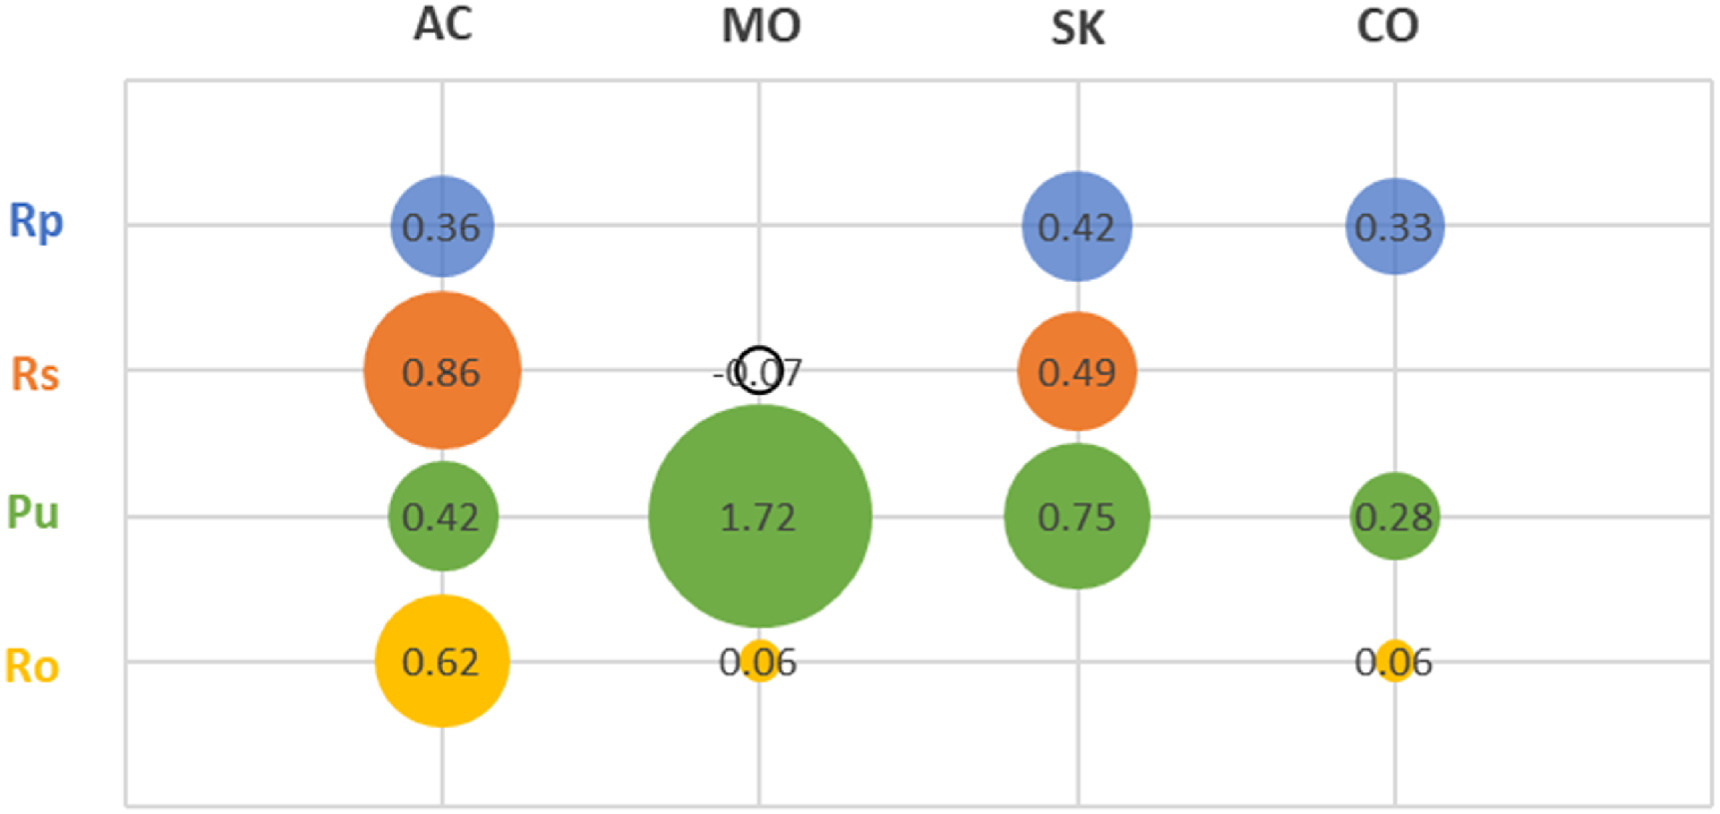
\includegraphics[width=0.7\linewidth]{results_meta_analysis.jpg}
  \captionof{figure}{Effectgroottes (\textit{Hedges' g}) van vier gamification-categorieen op vier leeruitkomsten in programmeeronderwijs \autocite{Zhan2022}.}
  \label{fig:zhan}
\end{center}

Niet elk element draagt evenveel bij. Puzzels en uitdagingen scoren het sterkst op motivatie (\(g \approx 1{,}72\)), terwijl rollenspel en verhaal nauwelijks effect hebben (\(g \approx 0{,}06\)). Dat verantwoordt de keuze om \textit{Learn COBOL} op te bouwen rond uitdagingen met snelle feedback en prestatiebeloningen. Omdat de PoC die kerncomponenten implementeert, is een effect in dezelfde grootteorde aannemelijk. Dit blijft een verwachting, want er werden geen metingen op deelnemers uitgevoerd.

%==============================================================================
\section{Conclusie}

Op basis van de literatuurevaluatie is het aannemelijk dat de gamification-elementen in \textit{Learn COBOL} een positief effect hebben op motivatie en leerwinst van junior developers. De bijdrage is viervoudig: een theoretisch kader, een functionele Proof-of-Concept, een literatuurevaluatie die elke ontwerpkeuze onderbouwt, en een herbruikbaar pilotontwerp. Een rechtstreekse, kwantitatieve vergelijking met een papieren cursus werd niet uitgevoerd.

%==============================================================================
\section{Toekomstig onderzoek}

De voornaamste aanbeveling is het uitvoeren van het uitgewerkte pilotontwerp. Daarin leren twee groepen junioren elk een dag COBOL, de ene via \textit{Learn COBOL} en de andere via een papieren cursus met dezelfde zeven thema's, gevolgd door een gedeelde kennistest. Het verschil tussen beide groepsgemiddelden zou de leer-effectiviteit empirisch toetsen.

%==============================================================================
\section{Referenties}
\begingroup
\renewcommand*{\bibfont}{\tiny}
\setlength{\bibitemsep}{0pt}
\noindent
\begin{minipage}[t]{0.68\linewidth}
  \printbibliography[heading=none]
\end{minipage}
\endgroup

\end{multicols}
\end{document}
